\chapter{Ensemble Learning}

Ensemble methods (also known as classifier combination methods) are used to improve classification accuracy by aggregating the predictions of multiple classifiers. An ensemble method constructs a set of \textbf{base classifiers} trained on the training set (sampled differently depending on the specific technique), and then predicts the output on instances by taking the majority vote.

The key idea that justifies the use of ensemble methods is the so-called \hyperlink{https://en.wikipedia.org/wiki/The_Wisdom_of_Crowds}{\textbf{wisdom of the crowds}}: the collective knowledge of a diverse and independent group of people usually exceeds that of a single individual. According to Surowiecki, there are five elements required to form a wise crowd: diversity of opinion, independence, decentralization, aggregation, and trust. These same elements can be applied to machine learning, where each ``individual'' in the crowd is a model.

To illustrate how a classifier's performance can be improved, consider the following example. \\
We have an ensemble of 25 binary classifiers, each with the same error rate $\varepsilon = 0.35$. The ensemble predicts the class label of a test instance by taking the majority vote on the predictions of the single classifiers. If these classifiers are perfectly identical, then they will all answer the same way on any test input, so the error rate of the ensemble will also be $\varepsilon$.

If instead the base classifiers are independent (their errors are uncorrelated), the ensemble makes a wrong prediction only if more than half of the base classifiers make a mistake; so the error rate of the ensemble is:
\begin{equation*}
    e = \sum_{i=13}^25 \binom{25}{i} \varepsilon^i (1-\varepsilon)^{25 - i} = 0.06
\end{equation*}
which is considerably lower than $\varepsilon$. \\\\
Ensemble classifiers can be constructed in many ways:
\begin{itemize}
    \item By manipulating the training set (bagging, boosting);
    \item By manipulating the input features (random forests);
    \item By manipulating the class labels. (error-correcting output coding).
\end{itemize}

\section{Bagging}

Bagging, which stands for Bootstrap AGGregatING, is a technique that samples with replacement from a data set according to a probability distribution. Given a dataset $X = \{x_1, \dots, x_n \}$, $m$ datasets o size $n$ are sampled from it, such that each record $x_i$ has $\frac{1}{n}$ probability of being extracted. Since replacement is used, the same record may appear multiple times in the same sample, while some records may not appear at all.
\begin{algorithm}
\caption{Bagging algorithm.}
\begin{algorithmic}[1]
    \State Let $k$ be the number of bootstrap samples.

    \For{$i=1$ to $k$}
        \State $D_i$ = Sample of size $N$.
        \State Train a base classifier $C_i$ on $D_i$.
    \EndFor
    \State $C^*(x) = \arg\max_y \sum_i \delta(C_i(x) = y)$
\end{algorithmic}
\end{algorithm} \\
In the above pseudocode, $\delta()$ is a function that returns 1 if its argument is true, 0 else.

Bagging improves generalization error by reducing the variance of the base classifiers. The performance of bagging depends on the stability of the base classifier: if a base classifier is unstable, bagging helps to reduce the errors associated with fluctuations in the training data, and if it is stable, the error of the ensemble will be mainly caused by bias of the base classifier.

\section{Boosting}

Boosting is an iterative procedure used to change the distribution of training examples for base classifiers, increasing weights for instances that are harder to learn. Initially, all instances in the original dataset are assigned a weight equal to $\frac{1}{n}$; a sample is selected (the same way bagging does, with replacement), and a classifier is built on it. All records that are incorrectly classified by this base classifier have their weight increased, while the ones that are correctly classified have theirs decreased. For the next step, another sample is obtained considering the new weights, and used to train a second model. After classifying those instances, their weights are updated, and this goes on until the desired number of boosting rounds is reached.

\subsection{AdaBoost}

In the AdaBoost algorithm, each base classifier $C_i$ is assigned an \textbf{importance}. It depends on the classifier's error rate, defined as:
\begin{equation*}
    \varepsilon_i = \dfrac{1}{l} \sum_{j=1}^l w_j \delta(C_i(x_j) \neq y_i)
\end{equation*}
where $\delta()$ is the same function seen in the bagging pseudocode. The importance is then calculated as:
\begin{equation*}
    \alpha_i = \dfrac{1}{2} \ln \left(\dfrac{1-\varepsilon_i}{\varepsilon_i}\right)
\end{equation*}
When the error is close to 0, the importance is a large positive value, while when the error is close to 1, the importance is a large negative value.
\begin{figure}[h]
    \centering
    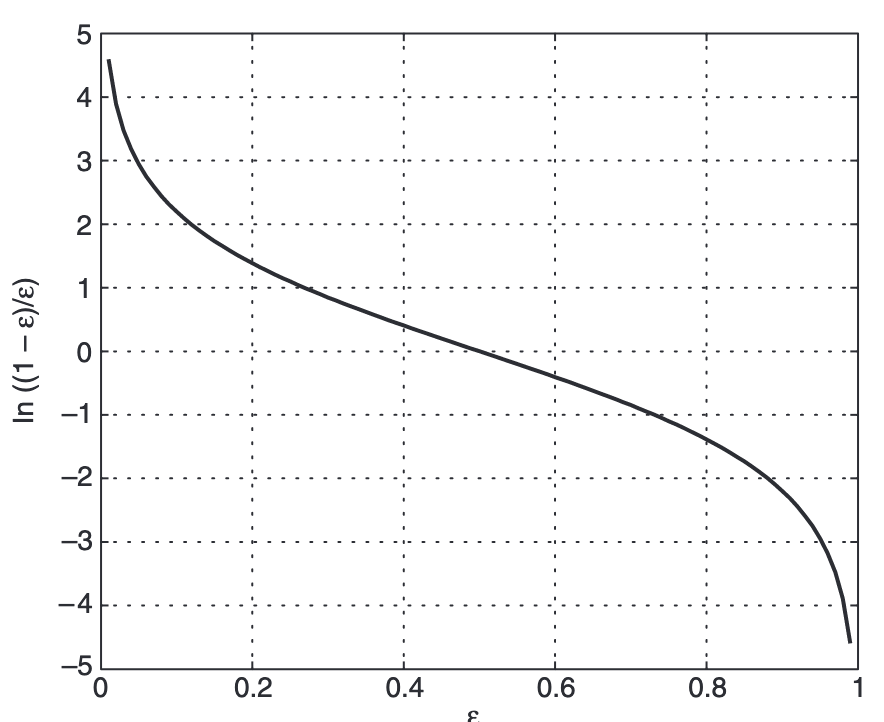
\includegraphics[width=0.4\linewidth]{img/importance_vs_errorrate.png}
    \caption{$\alpha$ as a function of the error rate.}
    \label{fig:importance-errorrate}
\end{figure} \\
The importance is used to update the weights of the training examples, as well. Given an example $x_i$, its corresponding weight at boosting round $j+1$ is:
\begin{equation*}
    w_i^{(j+1)} = \dfrac{w_i^{(j)}}{Z_j} \times \begin{cases}
        e^{-\alpha_j} & C_j(x_i) \neq y_i \\
        e^{\alpha_j} & C_j(x_i) \neq y_i 
    \end{cases}
\end{equation*}
$Z_j$ is the normalization factor, used to ensure that $\sum_i w_i^{(j+1)} = 1$. Using this formula, the weights of examples are increased for those incorrectly classified and decreased for those correctly classified, but the update is influenced by how ``good'' the classifier is. The classification is also influenced by the importance of the classifier:
\begin{equation*}
    C*(x) = \arg\max_y \sum_{j=1}^T \alpha_j \delta(C_j(x) = y)
\end{equation*}
This approach penalizes models with poor accuracy; additionally, if any intermediate boosting round produces an error rate higher than 50\%, the weights of the examples are reverted to their original value $\frac{1}{l}$, and the resampling procedure is repeated.

A default choice of models used by AdaBoost is \textbf{decision stumps}, a decision tree with only the root and two leaf nodes. By themselves, they are very weak learners, but together in an ensemble, they can be very powerful.

\section{Random Forest}

Random forests improve the performances of classifiers by constructing an ensemble of decorrelated decision trees. A key feature of this method is that each base model receives a sample that only selects a subset of the original attributes, usually of dimension $m' \approx \sqrt{m}$, or $m' \approx \log(m)$.

The decision trees used in a random forest are unpruned, as they are allowed to grow to their largest possible size until every leaf is pure. Hence, the base classifiers have lo bias but high variance.

This technique is one of the most accurate learning algorithms available, and is also efficient even on large datasets with thousands of input variables with no need for explicit variable deletion. It also provides an estimate of which variables are most important in classification, and generates an internal unbiased estimate of the generalization error as the forest building progresses.

\section{Gradient Boosting}

The goal of gradient boosting is to find the best hypothesis by expanding a starting function. In the case of regression, the functions are:
\begin{align*}
    &F_0(x) = \arg \min_{\gamma} \sum_{i=1}^n L(y_i, \gamma) = \mathrm{E}[y] \\
    &F_m(x) = F_{m-1}(x) + \left ( \arg \min_{h_m \in H} \sum_{i=1}^n L(y_i, F_{m-1}(x_i) + h_m(x_i)) \right ) (x)
\end{align*}
where $h_m$ is a base learner function, and the loss function is usually Squared Error Loss.

Choosing the best function at every step is a difficult optimization problem, so a steepest descent approach is used. After calculating $F_0(x)$ (which is simply the mean of all the target variable values), the following steps are repeated:
\begin{enumerate}
    \item The \textbf{pseudo-residuals} are calculated as:
    \begin{equation*}
        r_{im} = \left [ \dfrac{\partial L(y_i, F(x_i))}{\partial F_{m-1}(x_i)} \right ] \ \forall i = 1, \dots, n
    \end{equation*}
    (that is, the gradient).

    \item A base learner (usually a weak learner, e.g., a tree) is fit to the data, using the training set $\{x_i, r_{im}\}_{i=1}^n$. This creates a set of \textbf{terminal regions} $R_{jm}$ (in the case of trees, these regions correspond to the different leaves).

    \item The multiplier values $\gamma_{jm}$ are calculated as:
    \begin{equation*}
        \gamma_{jm} = \arg \min_{\gamma} \sum_{i:x_i \in R_{jm}} L(y_i, F_{m-1}(x_i) + \gamma)
    \end{equation*}
    These are the values that minimize the loss function within each leaf.

    \item The $m^{th}$ function is updated:
    \begin{equation*}
        F_m(x) = F_{m-1}(x) + \nu \sum_{j=1}^{J_m} \gamma_{jm} 1(x \in R_{jm}) 
    \end{equation*}
    where $\nu$ is a learning rate, and $1(\cdot)$ is an indicator function.
\end{enumerate}

When using gradient boosting for classification, the predictions are calculated as the log odds for the positive class. To transform it into a probability, the logistic function is used:
\begin{equation*}
    \dfrac{e^{log(p)}}{1+e^{log(p)}}
\end{equation*}
Pseudo-residuals are then calculated as the difference between the observed value and the predicted value. Since leaves will contain a mix of different values, the $\gamma_{jm}$ values are calculated as:
\begin{equation*}
    \gamma_{jm} = \dfrac{\sum_i \textit{Residual}_i}{\sum_i \left [ p_i(1-p_i) \right ]}
 \end{equation*}

\subsection{XGBoost}

XGBoost (eXtreme Gradient Boosting) is an implementation of regularized Gradient Boosting. The first step in the training phase is to choose a starting value; it can be anything, but by default it is 0.5 (regardless of wheter the problem is of regression or classification). Unlike Gradient Boosting which uses regular regression trees, XGBoost uses a special kind of model that is built as follows:
\begin{enumerate}
    \item The tree is initialized with a single leaf, containing all the residuals for all data points.
    
    \item For, regression, the \textbf{similarity score} is calculated as:
        \begin{equation*}
            \textit{Similarity Score} = \dfrac{(\sum_i \textit{Residual}_i)^2}{l + \lambda}
        \end{equation*}
    where $l$ is the number of residuals in the leaf, and $\lambda$ is a regularization term.
    For classification, the similarity score is calculated as:
    \begin{equation*}
        \textit{Similarity Score} = \dfrac{(\sum_i \textit{Residual}_i)^2}{\sum_i(p_i (1-p_i)) + \lambda}
    \end{equation*}

    \item Different splits are evaluated, and their similarity score is calculated: the one which improves the gain in similairity is chosen. This continues for each leaf until the desired tree depth is reached (by default, it is 6). Typically, the higher $\lambda$ is, the lower the similarity scores will be.
    
    \item Finally, the tree is pruned to avoid overfitting. A parameter $\gamma$ is set as a threshold, such that if a leaf's similarity is less than gamma, it is cut.
\end{enumerate}

\subsection{LightGBM}

LightGBM is another implementation of Gradient Boosting, which has faster training speeds than XGBoost, as well as higher accuracy. It uses a technique called \textbf{Histogram-based Gradient Boosting}, which discretizes continuous features into discrete bins (this approach also makes it so that LightGBM requires less memory). It also supports parallel and GPU learning.

When looking at the trees produced by this framework, they tend to show a lot of vertical growth, as opposed to those produced by XGBoost, which instead tend to grow horizontally.

LightGBM uses \textbf{Gradient-Based One-Side Sampling} (\textbf{GOSS}), which retains instances with larger gradients and samples those with lower gradients (basically focusing less on instances which have low training error). Another technique used is \textbf{Exclusive Feature Bundling} (\textbf{EFB}), a near lossless method to reduce the number of features, bundling features that are mutually exclusive (i.e., they never take zero values simultaneously) together.

\subsection{CatBoost}

CatBoost (Categorical Boosting) is a library that provides a gradient boosting framework. It uses \textbf{target encoding}, replacing each category of a variable with a number calculated from the distribution of the target labels for that category (e.g., the mean value). It uses \textbf{Symmetric Decision Trees}, which are balanced trees with the same splitting condition for all nodes at the same level.

\subsection{Explainable Boosting Machines}

Explainable Boosting Machines (EBM) are a type of Generalized Additive Model (GAM). The model trains one feature at a time, in a round-robin fashion at each iteration. They produce exact explanations about the model's predictions. 